\documentclass[12pt,a4paper]{article}
\usepackage{float}
\usepackage[spanish]{babel}
\usepackage{amsmath}
\usepackage{amssymb}
\usepackage{graphicx}
\usepackage{amsfonts}
\usepackage{textcomp}
\usepackage[utf8]{inputenx}
%\usepackage{algorithm2e}
\usepackage{listings}
\usepackage{pdfpages}
\usepackage{tabularx}
\usepackage{color,colortbl}
\usepackage{anysize}
\usepackage{fancyhdr}
\usepackage[nottoc]{tocbibind}
%\usepackage{caption}
\usepackage[font=footnotesize]{caption}
\definecolor{deepblue}{RGB}{0,0,153}
\definecolor{deepred}{RGB}{153,0,0}
\definecolor{deepgreen}{RGB}{51,102,0}
\definecolor{deepyellow}{RGB}{204,204,0}
\marginsize{2cm}{2cm}{0cm}{1.5cm} % depende de anysize

\definecolor{Gray}{gray}{0.85}
\newcolumntype{a}{>{\columncolor{Gray}}c}


\lstset{ %
			language=Python,
			basicstyle=\footnotesize,
			numbers=left,
			stepnumber=1,
			numbersep=4pt,
			tabsize=2,
			otherkeywords={self}, 
			keywordstyle=\color{deepred},
			stringstyle=\color{deepgreen},
			commentstyle=\color{deepblue},
}
\usepackage{hyperref}
\hypersetup{
    colorlinks=true,
    citecolor=black,
    filecolor=black,
    linkcolor=black,
    urlcolor=black,
    linktoc=all
}


%\title{Multímetros en Corriente Continua}
\title{Cuestionario Fisica III \\ Radiación}
\author{
        Alejandro Pernin
}
\date{\today}
%\pagestyle{fancy}
\lhead{Facultad de Ingenieria}
\rhead{Fisica III D - 62.16 - Grupo T07}


\begin{document}
	%\includepdf{caratula.pdf}

	\maketitle

	%\newpage
	%\tableofcontents

	% Item A
	\section{}\label{1}
		\textit{
		Graficar por computadora y en un mismo gráfico los espectros de radiación en función
		de lambda de un cuerpo negro a las temperaturas: 400, 800 y 1200 \textdegree C. Indicar en el gráfico
		(en una escala que permita distinguir las formas de las tres curvas) el rango visible (4000 –
		7500 Å) y la posición de las longitudes de onda para las cuales se alcanzan los máximos de
		intensidad. Hacer otro gráfico en el rango visible.
		}



		\subsection{Todo el rango}
			\begin{figure}[H]
				\centering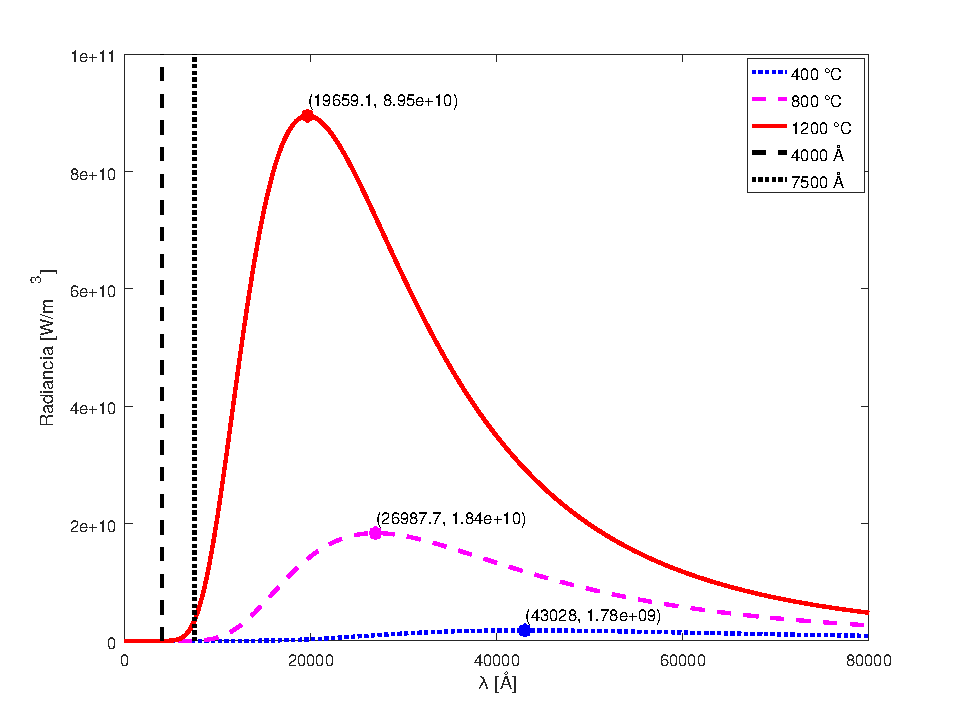
\includegraphics[scale=1]{images/todo.pdf}\caption{Radiancia espectral a 400, 800 y 1200 \textdegree C}
			\end{figure}
	
		\subsection{Rango visible}
			\begin{figure}[H]
					\centering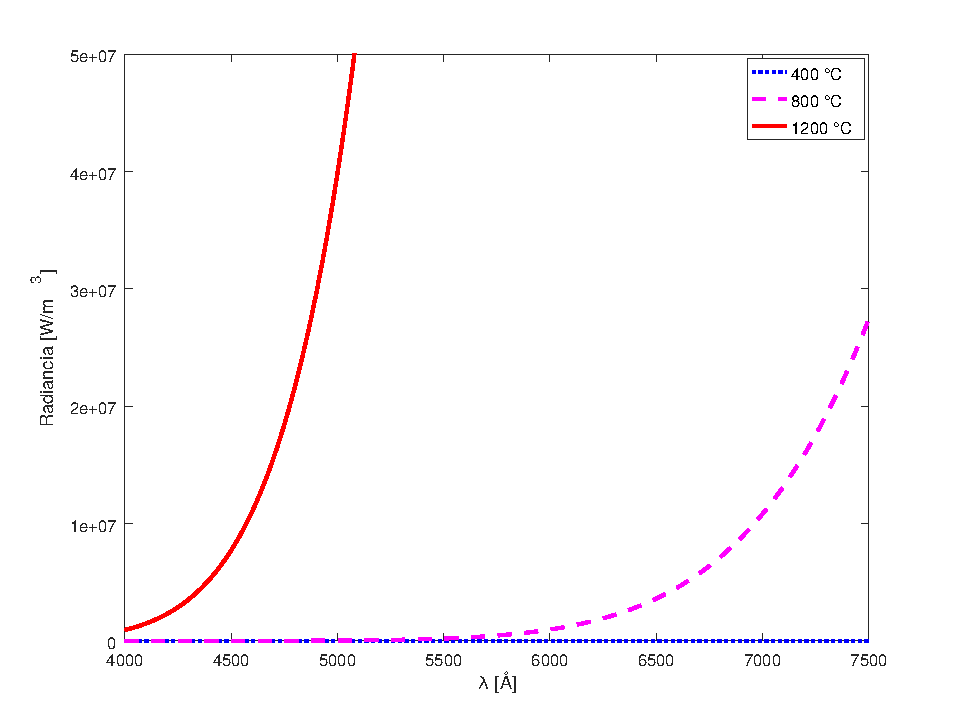
\includegraphics[scale=1]{images/visible.pdf}\caption{Radiancia espectral a 400, 800 y 1200 \textdegree C en el rango visible}
			\end{figure}

	%Item B
	\section{}
		\textit{
		Calcular la radiancia espectral a los 1600 nm (R(1600nm,T)) para cada una de las
		temperaturas del punto \ref{1}
		}

		\begin{align*}
			R(\lambda, 400 ^{\circ}C) = 5.66 * 10^7 \frac{W}{m^3} d\lambda \\
			R(\lambda, 800 ^{\circ}C) = 8.23 * 10^9 \frac{W}{m^3} d\lambda \\
			R(\lambda, 1200 ^{\circ}C) = 8.01 * 10^{10} \frac{W}{m^3} d\lambda \\
		\end{align*}

	%Item C
	\section{}
		\textit{Calcular la radiancia en el rango visible para cada una de las temperaturas del punto
		\ref{1}. Resolver “exactamente” utilizando algún método numérico y la aproximación del
		rectángulo. Comparar ambos resultados.
		}
		\\

		Para los cálculos se empleó una aproximación por rectángulos. Como aproximación se utilizó un sólo rectángulos,
		como metodo numérico exacto se utilizaron 10.000.

		\begin{center}
					
			{\footnotesize \begin{tabular}{ |c|c|c|c|}
		
			\hline
			Temperatura [$^{\circ}C$] & Aproximación [$\frac{W}{m^2}$]& Exacta [$\frac{W}{m^2}$] & Error Relativo \\ \hline
			400 \cellcolor{Gray} & $1.52 * 10^{-7}$ & $1.97 * 10^{-5}$ & 99.23\%\\ \hline
			800 \cellcolor{Gray} & $0.158$ & $1.37$ & 88.47\%\\ \hline
			1200 \cellcolor{Gray} & $88.34$ & $256.61$ & 65.57\%\\ \hline
			\end{tabular}}
		\end{center}

	%Item D
	\section{}\label{sec_d}
		\textit{
		Explicar brevemente qué es un pirómetro, cómo funciona un pirómetro IR y qué leyes de radiación de cuerpo negro se utiliza en la determinación de la temperatura.
		}

		Un pirómetro es un dispositivo capaz de medir la temperatura de un cuerpo sin estar en contacto con el mismo. 

		\subsection{Pirómetro Óptico}
			Un pirómetro óptico emplea al ojo humano para la medición. Posee un filamento calibrado en su interior, el cuál se aumenta la temperatura mediante el paso de corriente. La superposición del filamento con la visión del objetivo, permite observar cuando ambos objetos (filamento y objetivo) se encuentran a una temperatura similar.

			\begin{figure}[H]
				\centering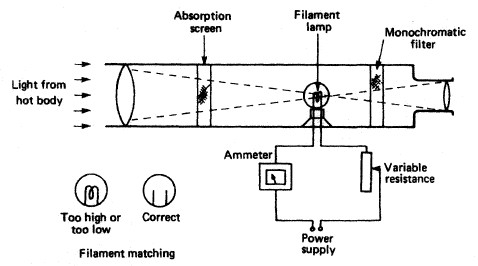
\includegraphics[scale=.8]{images/optical-pyrometer.jpg}\caption{Ejemplo pirómetro óptico}
			\end{figure}

			\begin{figure}[H]
				\centering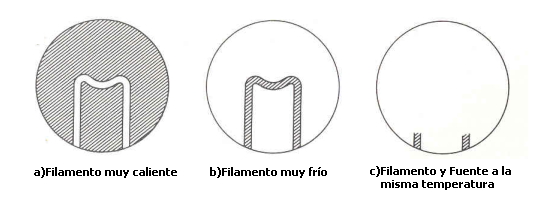
\includegraphics[scale=0.75]{images/fila.png}\caption{Ejemplo pirómetro óptico}
			\end{figure}

		\subsection{Pirómetro Infrarrojo}
			Los pirómetros infrarojos se valen de la radiación emitida por el cuerpo a medir, enfocándose en el espectro infrarrojo mediante filtros.

			\begin{figure}[H]
				\centering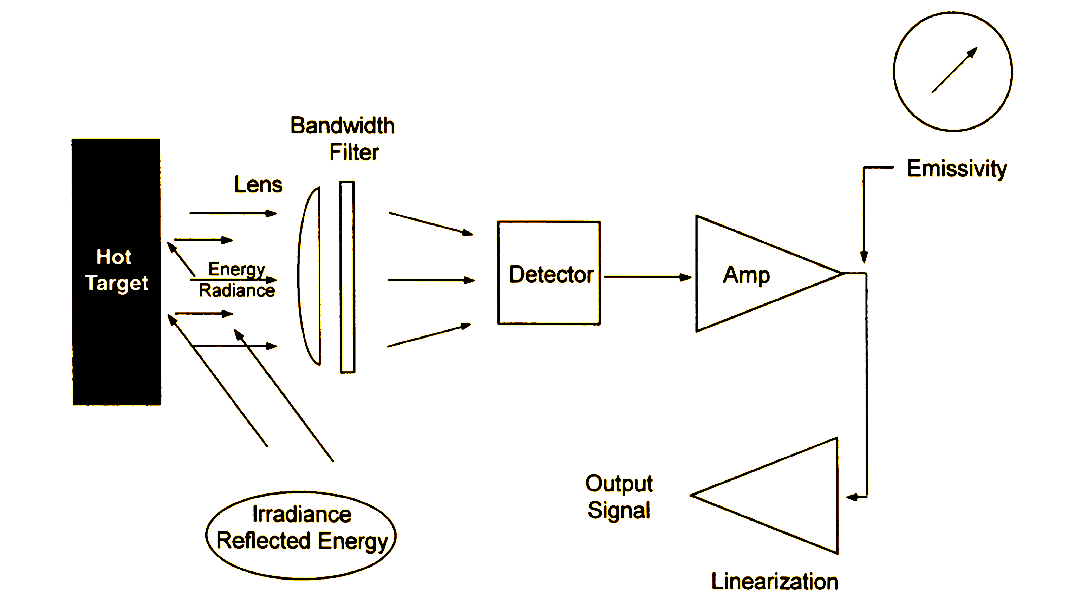
\includegraphics[scale=0.3]{images/ir-pyro.png}\caption{Pirómetro Infrarrojo}
			\end{figure}

			Estos pirómetros basan su funcionamiento en la Ley de Plank \footnote{Ver fórmula \ref{f_planck}}, dado que los pirómetros operan sobre un espectro acotado de longitudes de onda, la fórmula de la radiancia se puede describir como

			\begin{equation}
				R(T) = \frac{C_1}{e^{\frac{C_2}{T}}-1}
			\end{equation}

			donde $C_1$ y $C_2$ son valores de calibración del pirómetro. Siendo que el pirómetro es capaz de obtener el valor de la radiancia espectral, podemos despejar la temperatura

			\begin{equation}\label{temp_ir_pyro}
				T = \frac{C_2}{ln\left( \frac{C_1}{R_T} + 1\right)}
			\end{equation}

	% Item E
	\section{}
		\textit{
		De acuerdo a lo visto en el punto anterior, comentar qué magnitudes experimentales es necesario conocer para poder medir la temperatura con un pirómetro IR.
		}

		Como vimos en la fórmula \ref{temp_ir_pyro}, precisamos de los valores de calibración $C_1$ y $C_2$, así como también la lectura de la radiancia espectral $R_T$.

	% Item F
	\section{}\label{item_f}
		\textit{
		Explicar cómo es la dependencia de la resistencia con la temperatura (a altas
		temperaturas) en materiales \textbf{conductores}, dar la expresión matemática de dicha
		dependencia y explicar brevemente su origen físico.
		}
		\\\\
		La resistencia de un material es la medida de que tanto el material se opone al flujo de electrones a través de dicho material. Se encuentra fuertemente ligada a la \textit{resistividad} o resistencia específica del material, así como también a la temperatura a la que se encuentra.

		Considerando un material conductor con sección transversal uniforme, podemos definir la resistencia como

		\begin{equation}\label{resistencia}
			R = \rho \frac{l}{A}
		\end{equation}

		donde $\rho$ es la \textit{resistividad} del material, $l$ el largo del material y $A$ el área de la sección. Aumentar el área de la sección reducirá la resistencia dado que habrá mayor flujo de electrones. Aumentar la longitud del material, por el contrario, hará que los electrones deban recorrer mayor longitud y en consecuencia, se ven mas obtaculizados a fluir.

		La relación entre la resistencia y la temperatura se da mediante la resistividad, cuya dependencia con la temperatura se da mediante\footnote{Para pequeños intervalos de temperaturas (hasta 100 \textdegree C)}

		\begin{equation}\label{resistividad}
			\rho(T) = \rho_{0} \left[ 1 + \alpha (T - T_0) \right]
		\end{equation}

		donde $T_0$ es una temperatura de referencia, $\rho_0$ la resistividad a dicha temperatura de referencia y $\alpha$ una constante de ajuste también dependiente de $T_0$. Siendo $\alpha > 0$ para la mayoría de los materiales \footnote{Ver apéndice Resistencia \ref{apendice_resistencia}} podemos afirmar que la resistividad aumenta linealmente con la temperatura. Esto es dado a que un aumento en la temperatura provoca que los iones del conductor vibren con mayor amplitud, haciendo más probable que un electrón en movimiento colisione con un ion; dificultando el flujo de electrones.

		Combinando las ecuaciones \ref{resistencia} y \ref{resistividad}, podemos obtener la expresión de la resistencia dependiendo de la temperatura

		\begin{equation}
			R(t) = \rho_0 \frac{l \left[ 1 + \alpha (T - T_0) \right] }{A}
		\end{equation}
		
		Considerando que $l$ y $A$ no se modifican para un material, podemos utilizar $R_0 = \rho_0 \, l/A$, quedando

		\begin{equation}
			R(t) = R_0 \left[ 1 + \alpha (T - T_0) \right]
		\end{equation}

	% Item G
	\section{}
		\textit{
			Ídem para materiales \textbf{semiconductores}.
		}

		La resistividad de los semiconductores disminuye con el aumento de la temperatura. Los electrones son llevados a la banda de conducción mediante energia térmica, dejando agujeros en la banda de valencia.

		La dependencia con la temperatura está dada por

		\begin{equation}
			R(T) = R_0 \: e^{\left(\displaystyle \beta \left[\frac{1}{T} - \frac{1}{T_0} \right] \right)}
		\end{equation}

		donde análogamente a lo visto en la sección \ref{item_f}, $R_0$ y $\beta$ son valores tomados a la temperatura de referencia $T_0$.

\newpage
\section{Apéndice}
	\subsection{Radiación}\label{apendice_radiacion}
		Para los cálculos, se emplearon las siguientes funciones y constantes.
	
		Ley de Plank
			\begin{equation}\label{f_planck}
				\displaystyle R_{\lambda}(\lambda, T) = \frac{2 \pi h c^2}{\lambda ^5} \frac{\epsilon}{e^ {\frac{hc}{\lambda k T}} - 1}
			\end{equation}
	
			Constante de Plank: $h = 6.626 * 10^{-34} Js$
			
			Velocidad de la Luz: $c = 2.998 * 10^8 \frac{m}{s}$
			
			Constante de Boltzmann: $k = 1.3807 * 10^{-23} \frac{J}{K}$
			
			Emisividad: $\epsilon \in [0,1]$
			
			Temperatura: $[T] = K$
			
		Longitud de Onda: $[\lambda] = m$

	\subsection{Resistencia}\label{apendice_resistencia}
		\begin{figure}[H]
			\centering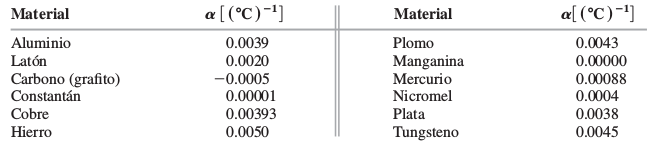
\includegraphics[scale=0.75]{images/tabla_coeficiente_resistividad.png}\caption{Coeficientes de temperatura de la resistividad}
		\end{figure}

\begin{thebibliography}{1}
	\bibitem{Resistencia} 
		Sears, Zemansky.
		\textit{Física Universitaria con Física Moderna Vol 2}.
		Addison-Wesley, 2009.

	\bibitem{Pirometro}
		\textit{The Fundamentals of Infrared Temperature Measurement}.
		\href{www.pyrometer.com}{www.pyrometer.com}

	\bibitem{Pirometro2}
		\textit{Selecting Non Contact Pyrometers and Infrared Thermometers}.
		\href{www.pyrometer.com}{www.pyrometer.com}

\end{thebibliography}

\end{document}
